\documentclass[10pt,a4paper]{article}
\usepackage[utf8]{inputenc}
\usepackage{amsmath}
\usepackage{amsthm}
\usepackage{amsfonts}
\usepackage{amssymb}


\usepackage[spanish]{babel}

\usepackage{graphicx}
\usepackage[margin=1.1in]{geometry}


\newcommand{\N}{\mathbb{N}}
\newcommand{\Z}{\mathbb{Z}}
\newcommand{\Q}{\mathbb{Q}}
\newcommand{\R}{\mathbb{R}}
\newcommand{\C}{\mathbb{C}}
\newcommand{\Rr}{\mathcal{R}}
\newcommand{\G}{\Gamma}
\newcommand{\ra}{\rightarrow}
\newcommand{\bra}{\textcolor{blue}{\longrightarrow}}
\newcommand{\bla}{\textcolor{blue}{\longleftarrow}}
\newcommand{\rra}{\textcolor{red}{\longrightarrow}}
\newcommand{\rla}{\textcolor{red}{\longleftarrow}}
\newcommand{\Ra}{\Rightarrow}
\renewcommand{\S}{\Sigma}
\newcommand{\bz}{\bm{0}}
\newcommand{\bo}{\bm{1}}

\newcommand{\peq}{\preceq}

\renewcommand{\a}{\alpha}
\renewcommand{\b}{\beta}
\newcommand{\g}{\gamma}

\renewcommand{\L}{\mathcal{L}}
\newcommand{\I}{\mathcal{I}}
\newcommand{\genericfol}{\L = (\mathcal{F})}
\newcommand{\U}{\mathcal{U}}

\title{Semántica y consecuencia lógica: intuición, usando gatos \\
\large Lógica computacional - ITBA
}
\author{Marcelo Lynch\footnote{mlynch@itba.edu.ar}}
\date{}


\begin{document}
\maketitle

\section*{Sobre la ``verdad'' de una fórmula}
La introducción de una semántica (``significado'') para las fórmulas, que en principio definimos como elementos puramente sintácticos (cadenas de símbolos) la hicimos a través de \textbf{valuaciones}: funciones que a cada fórmula hace valer $1$ o $0$. Rápidamente identificamos al $1$ como ``verdadero'' y al $0$ como ``falso'', y de hecho tanto la definición de lo que vale una valuación como los razonamientos los hacemos con eso en la cabeza.\\

Claro, la definición de lo que vale una valuación en una fórmula con conectivos está hecha para que funcione igual que nuestra noción de ``lo que significa ese conectivo'': que $v(\a \land \b) = \text{mín \{} v(\a), v(\b) \}$ en definitiva es porque es la manera conveniente de decir ``quiero que la conjunción sea \textit{verdadera} solo cuando ambos miembros lo sean''. \\
 
Desarrollar esta intuición cuando nos encontramos con esas definiciones en esta materia es bastante natural, quizás porque ya nos habíamos encontrado antes con los símbolos $\land$, $\vee$, $\ra$ interpretados como ``y'', ``o'', ``implica'', haciendo demostraciones en materias anteriores. Así, no nos es dificil ver ``qué oración'' es la que ``dice'' cada fórmula: $(p_1 \ra (p_2 \vee p_3))$ la leemos como ``$p_1$ implica $p_2$ o $p_3$'' y sabemos que esta fórmula es \textit{verdadera} dependiendo de si son \textit{verdaderas} o no $p_1, p_2, p_3$. Pero: ¿qué significa en sí misma la fórmula $p_1$? ¿Que significa decir que ``$p_1$ es verdad''? La respuesta rápida es: ``bueno, es si la valuación en $p_1$ vale $1$'', pero la contrapregunta a eso es: ¿y qué significa \textit{intuitivamente} una valuación? (¿hay una intuición posible?). \\

En lo que sigue quiero mostrar una forma de des-abstraer (!) un poco las definiciones, interpretándolas en términos de la verdad o falsedad de hechos concretos (en este caso los hechos serán la actividad de ciertos gatitos). Así es justamente (aunque en el sentido inverso) cómo se usa la lógica proposicional en la práctica: se hacen corresponder con variables proposicionales a ciertos ``hechos'' que podrían ser verdaderos o falsos (aunque no suelen tener que ver con gatitos\footnote{Para un ejemplo más razonable, se puede ver el apunte ``Una aplicación del teorema de compacidad''.}). Con esta \textit{concretización} conceptual también se puede bajar un poco más a tierra el concepto de conjunto de consecuencias y sus distintas propiedades, dando una intuición más directa que evidencia la motivación de las definiciones.


\section*{Valuaciones como posibles mundos de gatos dormilones}


Como ya sabemos, la verdad o falsedad de cada variable está dada por la valuación que elegimos, entonces elegir una valuación es en definitiva elegir elegir que \textit{ciertas cosas} son verdaderas y \textit{ciertas cosas}  son falsas, donde esas ``ciertas cosas'' están representadas por las infinitas variables.\\

La forma de hacer esto más concreto es asociar las variables a ciertos \textit{hechos} que podrían ser verdaderos o falsos en un  ``estado posible del mundo''. Podriamos elegir cualquier mundo que tenga ``hechos'' verdaderos y falsos que nos interesan (como el mundo real), pero para hacerlo fácil elijamos un mundo que sea simple: para lo que sigue vamos a trabajar en un universo que \textbf{lo único que tiene es tiene infinitos (pero numerables) gatos al sol}.\\

Cada gato tiene un número natural asociado (los podemos coordinar con $\N$), y puede estar dormido o despierto (el sol está especial para dormir la siesta, pero también hay que estirar las patas cada tanto).  En adelante cuando hablemos del \textit{mundo} vamos a estar hablando de este mundo, en donde \textit{solo importa si cada gato está despierto o dormido}. \\

Supongamos ahora que frenamos el tiempo en este universo y nos fijamos en como está la cosa. En ese instante cada gato tiene un estado definido: o está despierto o está dormido. Así, podemos definir una función $f: Var \ra \{0,1\}$ tal que $f(p_i) = 1$ si el gato $i$ está despierto, y $0$ el gato $i$ está dormido. O sea que podemos ``leer'' la variable $p_i$ como ``el gato $i$ está despierto'', y hacerla valer $1$ si esto es verdad. \\


\begin{figure}[h!]
\centering
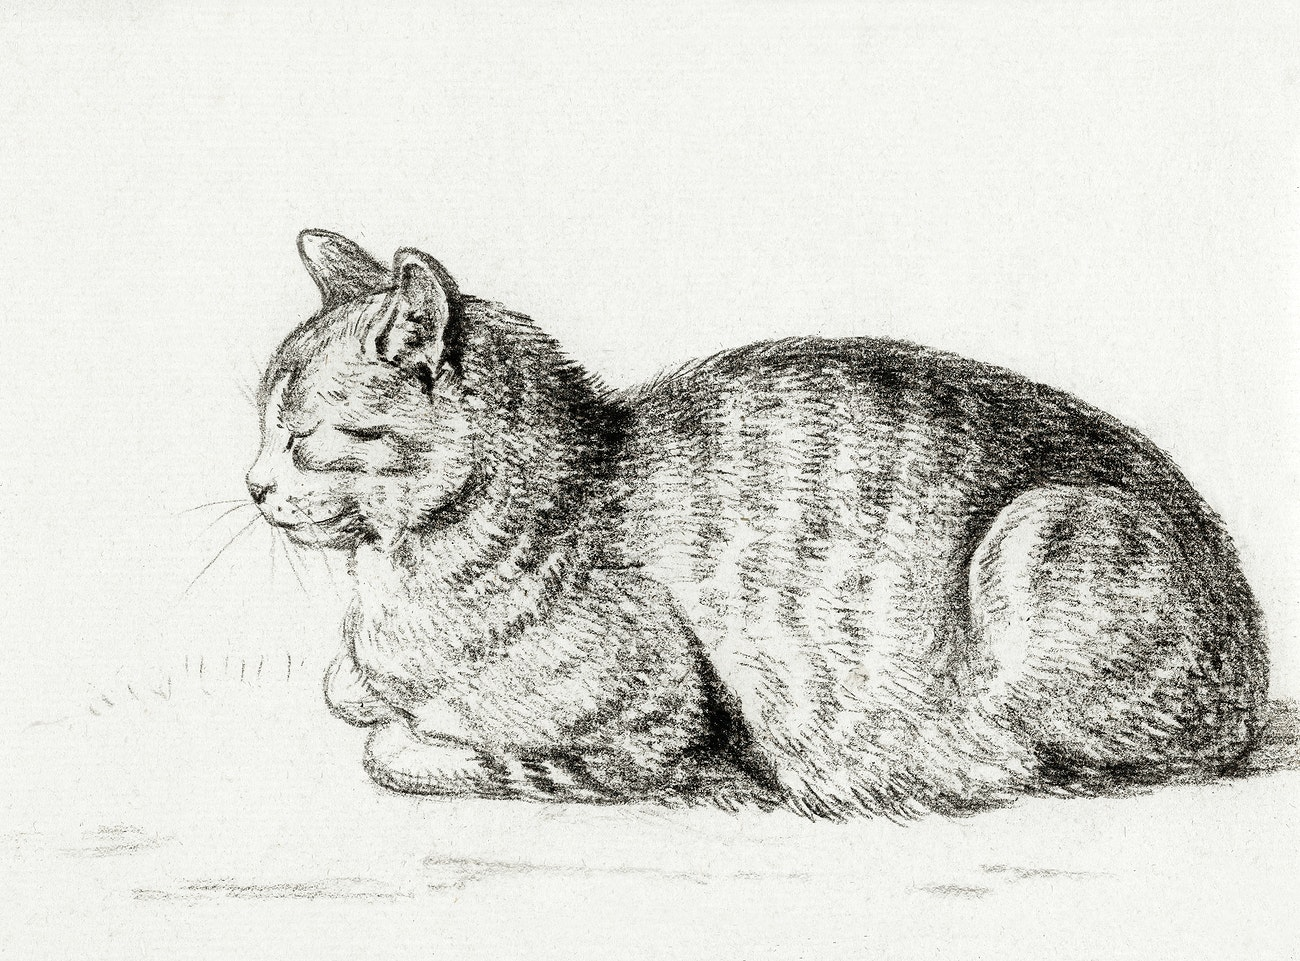
\includegraphics[scale=0.15]{gato}
\caption{$f(p_i) = 0$ cuando el gato $i$ está dormido}
\end{figure}


Con esta idea podemos pensar a una función $Var \ra \{0,1\}$ como un estado posible de este universo felino: \textbf{frenar el tiempo en distintos momentos nos puede dar distintas funciones, y cada función se puede pensar como una configuración distinta de sueño y vigilia de los infinitos gatos}.\\


En esta analogía entonces \textbf{las fórmulas} son todas las cosas que podemos decir usando el estado de cada gato individual (las variables) y los conectivos que tenemos: $(p_1 \land p_3)$ es ``el gato $1$ está despierto y el gato $3$ está despierto'', $(p_4 \ra \neg p_0)$ es ``si el gato $4$ está despierto, entonces el gato $0$ no está despierto''. Entonces las fórmulas son  oraciones que dicen cosas sobre el estado de los gatos\footnote{No podemos decir todo lo que queramos: por ejemplo, es imposible decir ``todos los gatos están despiertos'' porque esto sería una fórmula de longitud infinita} y podrían ser verdaderas o falsas, dependiendo de cómo esté el mundo. \\

Y una valuación $v : \text{Form} \ra \{ 0, 1 \}$ entonces se puede pensar como un oráculo de la ``verdad o mentira'' de cualquiera de estas oraciones, \textbf{en un momento en que el universo de gatos está descrito por la restricción de $v$ a las variables}. Es decir, un oráculo que puede darme el valor de verdad (en ese momento particular de gatitos) de cualquier oración (fórmula) de las que podemos armar. \\


De nuevo: una valuación me \textbf{define un estado del mundo} y determina qué cosas (de las que podemos expresar a partir de nuestros ``hechos'' individuales, o sea las variables) son verdaderas y son falsas en ese estado. Así, una tautología sería algo que es verdadero (``vale $1$'') en todos los estados posibles del mundo (``para cualquier valuación'') y una contradicción es algo que es falso en todos los estados posibles del mundo. Y una contingencia es una oración que dice algo que podría ser verdadero o falso... depende del estado del mundo en el que estemos parados. \\


\textbf{\textbf{Observación}:} Pensandolo así es fácil convencerse de dos propiedades que tenemos de las valuaciones: primero, que la valuación va a estar únicamente determinada por lo que vale en las variables: lo unico que importa en este mundo es si los gatos están despiertos o dormidos, la verdad del resto de las ``oraciones'' (fórmulas) va a quedar determinada por ``cómo está el mundo''. Segundo, que el valor de verdad de una fórmula queda determinado unicamente por el valor en las variables involucradas en esa fórmula: ¿qué me importa el gato $34$ si la oración que le pregunto al oráculo solo habla sobre los gatos $6$, $28$ y $1995$?


\section*{Satisfactibilidad}
Una fórmula $\a$ es satisfacible si existe una valuación $v$ que la satisface, es decir que cumple $v(\a) = 1$. En la analogía, las definiciones se vuelven:
\begin{itemize}
\item \textit{$v(\a) = 1$ si lo que dice $\a$ es verdadero en el estado del mundo descrito por $v$ } 
\item $\a$ \textit{es satisfacible si existe un posible estado del mundo en el que lo que dice es verdadero }
\end{itemize}

Asi, $(p_0 \land \neg p_0)$ no es satisfacible, porque de ninguna manera podría ser que el gato $0$ esté despierto y dormido al mismo tiempo. \\

Una valuación $v$ satisface a un conjunto $\G \subset Form$ si satisface a toda $\a \in \G$. En la analogía, tenemos:

\begin{itemize}
\item $v(\G) = 1$ \textit{si todas las oraciones de $\G$ son verdad en el estado del mundo descrito por $v$ } 
\item $\G$ \textit{es satisfacible si es posible un estado del mundo en el que todas las oraciones de $\G$ sean ciertas } 
\end{itemize}


\section*{Consecuencia lógica}
Cotidianamente decimos que $A$ es consecuencia de $B$ si ``que pase $B$ hace que pase $A$''. Cuando hablamos de consecuenca \textit{lógica} lo que nos interesa es este concepto aplicado a nociones sobre la verdad o falsedad de oraciones. Coloquialmente, $Q$ es una consecuencia lógica de $P$ si siempre que $P$ es verdadero, $Q$ también lo es.\\

La definición del conjunto de consecuencias de un conjunto de fórmulas $\G$ es: \[ C(\G) = \{ \a : v(\G) = 1 \Ra v(\a) = 1 \} \]

Intuitivamente, lo que me está diciendo esta definición es que $\a \in C(\G)$ si y solo si $\a$ es verdadera en cualquier estado del mundo que (``para cualquier valuación que'') haga que $\G$ tenga todas fórmulas verdaderas (``satisface $\G$''). \\

De otra manera: supongamos que nos dan una lista de fórmulas $\G$ y nos dicen: \textit{en este momento todo esto es verdadero en el mundo}. La pregunta es: ¿\textit{\textbf{qué otras cosas son verdaderas si $\G$ lo es}}? O: \textit{\textbf{¿qué más se desprende\footnote{Voy a usar la palabra \textit{desprender} para este proceso de ``averiguar que algo es verdadero a partir de lo que ya sabemos que es verdadero''. Una palabra más natural sería \textit{deducir}, pero la evito porque ya la usamos en la parte de axiomática. Igual, como demostramos en clase, los conceptos coinciden, porque $\a \in C(\G) \iff \G \vdash \a$} de saber que $\G$ es verdad?}} Todo esto (junto con $\G$) constituye $C(\G)$.\\


\textbf{Ejemplo}: Consideremos $\G = \{ p_0, (p_0 \ra \neg p_1), (p_2 \land p_3) \}$. Supongamos un estado del mundo en el que todo lo que dice $\G$ es verdadero. Entonces sabemos (y solo sabemos esto en principio) que son ciertas las siguientes:

\begin{itemize}
\item ``El gato $0$ está despierto''
\item ``Si el gato $0$ está despierto, entonces el gato $1$ no está despierto''
\item ``El gato 2 está despierto y el gato 3 está despierto''
\end{itemize}

¿Qué cosas \textbf{estamos seguros} que serán verdad \textbf{siempre que todo esto sea verdad}? Algunos ejemplos:

\begin{itemize}
\item ``El gato $1$ no está despierto'' (por lo primero y lo segundo anterior)
\item ``El gato $2$ está despierto''
\item ``El gato $3$ está despierto''
\end{itemize}
 
Traduciendo a fórmulas: $\{ \neg p_1, p_2, p_3 \} \subset C(\G)$.\\

\textbf{Demostración} (comparar con lo anterior): Sea $v$ valuación tal que $v(\G) = 1$, entonces:

\begin{enumerate}
\item $v(p_0) = 1$
\item $v(p_0 \ra \neg p_1) = 1$
\item $v(p_2 \land p_3) = 1$
\end{enumerate}

Entonces:

\begin{itemize}
\item $v(p_0 \ra \neg p_1) = 1$ o sea $\textit{máx \{} 1 - \underbrace{v(p_0)}_{=1}, v(\neg p_1) \} = 1$, es decir $v(\neg p_1) = 1$
\item $v(p_2 \land p_3) = 1$, entonces $v(p_2) = 1$
\item $v(p_2 \land p_3) = 1$, entonces $v(p_3) = 1$
\end{itemize}

Es decir probamos que si $v(\G) = 1 \Ra v(\a) = 1$ para $\a \in \{ \neg p_1, p_2, p_3 \}$, es decir que $\{ \neg p_1, p_2, p_3 \} \subset C(\G) \qed$.\\
 

\textbf{Observación:} Con esta intuición (``$C(\G)$ es todo lo que estamos seguros que será verdad siempre que estemos en un estado del mundo en el que $\G$ es verdad'') es claro que $C(\G)$ incluye a las tautologías para todo $\G$ (porque siempre estamos seguros de que las tautologías son verdad), pero quizás se escapa el hecho de que $C(\G) = Form$ si $\G$ es insatisfacible. Lo que pasa es que si $\G$ es insatisfacible entonces no será verdad \textit{en ningún estado posible del mundo}, entonces si asumimos que lo es... ¡podríamos asegurar cualquier cosa! (O: ``si el antecedente es falso cualquier  implicación es verdadera'').


\subsection*{Propiedades de las consecuencias, intuitivamente}


\vspace{10px}
\fbox{
\noindent
\begin{minipage}{0.95\linewidth}
\hspace{1pt}
\textbf{Recomendación:} No leer lo que sigue antes de intentar por lo menos una vez de resolver los ejercicios sobre consecuencias de la guía 3.
\end{minipage}
}
\vspace{10px}


\vspace{10px}
\fbox{
\noindent
\begin{minipage}{0.95\linewidth}
\hspace{1pt}
\textbf{Recordatorio:} Lo que viene a continuación es simplemente una forma intuitiva de razonar las propiedades, que puede servir para razonar sobre otras que uno se pueda encontrar en el camino. Nada de esto reemplaza a una demostración utilizando las definiciones (y la intuición siempre puede fallar), pero puede servir para saber por dónde encararla.
\end{minipage}
}
\vspace{10px}


Me gusta pensar en la obtención del conjunto de consecuencias de $\G$ como el resultado del siguiente procedimiento:

\begin{enumerate}
\item Imprimo las fórmulas de $\G$ en una hoja (posiblemente infinita)
\item Llamo a alguno de mis ayudantes, que tienen infinita paciencia, y le digo: suponete que esta lista de cosas sobre los gatos ($\G$) es cierta: necesito que me traigas en una lista todas las cosas que \textbf{seguro, seguro} son ciertas en un mundo en el que lo unico que sabés es que lo que te entrego es cierto\footnote{Faltaría decir: ``A menos que lo que te estoy dando sea insatisfacible, en cuyo caso traeme todas las fórmulas''. En general para los ejemplos que escribo acá la intuición que doy funciona si los conjuntos son satisfacibles: siempre hay que analizar el caso aparte ``¿qué pasa si alguno de los conjuntos con los que trabajo es insatisfacible?'', que suele ser claro porque las consecuencias se vuelven $Form$.\\}. 
\item Se pone a trabajar, haciendo razonamientos como los que hicimos en el ejemplo anterior a toda velocidad\footnote{Mis ayudantes también tienen infinita rapidez mental y mecanográfica\\}. Cada vez que logra \textit{desprender} algo nuevo como verdadero a partir de lo que yo le di, lo agrega a su lista como una consecuencia. Además, cada cosa que anota se transforma también en un nuevo ``dato'' que puede asumir verdadero para seguir trabajando.
\item Espero un tiempito: el ayudante es realmente minucioso y completará la lista con absolutamente todas las fórmulas que cumplen lo que le pedí.
\item El ayudante me trae la lista completa. En esa lista tengo $C(\G)$.
\end{enumerate}


Con esta versión ``procedimental'' de $C(\G)$, veamos cómo podemos intuitivamente atacar y convencernos de la verdad o falsedad de algunas propiedades (o afirmaciones falsas) sobre los conjuntos de consecuencias. Es importante volver a recordar que esto es puramente intuitivo: la demostración siempre debe hacerse con las definiciones formales.


\subsubsection*{\underline{Propiedad: $\G_1 \subset \G_2 \Ra C(\G_1) \subset C(\G_2)$}}
Como $\G_2$ tiene todo lo que dice $\G_1$ (y quizás más cosas), entonces claro que $C(\G_2)$, que es todo lo que se desprende de $\G_2$, incluirá a $C(\G_1)$, que es todo lo que se desprende de ``solamente'' $\G_1$. O bien: si yo le doy a mi ayudante la lista $\G_2$, ella a la vuelta me va a traer a algo que incluye todo lo que me traeria si sólo le doy $\G_1$, que es ``una parte'' de $\G_2$.
\vspace{20px}
\subsubsection*{\underline{Propiedad: $C(C(\G)) = C(\G)$}}
Tengo un conjunto $\G$. Quiero sus consecuencias: se las doy a un ayudante (``Por favor, traeme todo lo que es verdadero si $\G$ es verdadero''). Vuelve después de todo ese trabajo con $C(\G)$. \\ 

Inmediatamente le digo: tomá, te lo devuelvo, traéme todo lo que es cierto si esto que me acabas de traer es cierto (o sea: ``traeme $C(C(\G))$''). Pero eso lo ofende, y me dice: ``pero: ¡ya te traje todo lo que se puede desprender de ahí, si hubiera más cosas lo habría agregado antes de traertelo! Lo que me pedís es esa misma lista!''.\\

Efectivamente, no hay nada más que hacer: $C(\G)$ y $C(C(\G))$ son lo mismo.

\vspace{20px}
\subsubsection*{\underline{En general es falso que $C(\G_1 \cup \G_2) \subset C(\G_1) \cup C(\G_2)$ (ejercicio 5.1)}}

Supongamos que tengo dos listas de fórmulas, $\G_1$ y $\G_2$. Llamo a mis ayudantes, y a una le doy una copia de la lista $\G_1$ y le digo: traéme las consecuencias, $C(\G_1)$. Mientras ella va a hacer la lista de todas las cosas que son verdaderas sabiendo solamente $\G_1$, a otro ayudante le doy una copia de $\G_2$. Cuando vuelven con sus reportes ($C(\G_1)$ por un lado, $C(\G_2)$ por el otro) obtengo entonces $C(\G_1) \cup C(\G_2)$. Mientras tanto, yo tengo tanto $\G_1$ como $\G_2$ y puedo entonces obtener $C(\G_1 \cup \G_2)$ por mi lado\footnote{Podría darselo a un tercer ayudante, pero a veces están todos ocupados con otras cosas}. \\

Ahora bien: si la propiedad es verdadera:

\[ C(\G_1 \cup \G_2) \subset C(\G_1) \cup C(\G_2) \]

entonces \textbf{todo lo que yo haya desprendido de $\G_1 \cup \G_2$ está en alguna de las dos listas que me trajeron mis asistentes}: ¡pero cada uno de ellos tenía una porción de la información que tenía yo! ¿Cómo puede ser que siempre (si la propiedad vale, no importa quienes sean $\G_1, \G_2$) desprendan tanto o más que yo?\\

Por ejemplo quizás la lista $\G_1$ solo dice ``el gato $1$ está despierto'' ($\G_1 = \{ p_1 \}$), y la lista $\G_2$ solo dice ``el gato $13$ está dormido'' (o sea $\G_2 = \{ \neg p_{13}  \}$). Yo, que \textbf{sé las dos cosas}, puedo desprender la oración ``el gato $1$ está despierto \textbf{y} el gato $13$ está dormido'', o sea que $(p_1 \land \neg p_{13})$ es verdadero, pero es imposible que ninguno de mis dos asistentes tenga esto entre sus consecuencias ¡porque uno no sabe nada del gato $1$ y el otro no sabe nada del $13$!. \\

Dicho de otra forma (y formal entre paréntesis): puede existir un estado del mundo (``existe\footnote{En una demostración formal, habría que construirla.} una valuación $v$'') en el que el gato $1$ está despierto (``tal que $v$ satisface $\G_1$'') y el gato $13$ también, o sea que ``el gato $1$ está despierto \textbf{y} el gato $13$ está dormido'' es falso (``pero con $v(p_1 \land \neg p_{13}) = 0$, entonces $(p_1 \land \neg p_{13}) \not\in C(\G_1)$'').

\vspace{20px}
\subsubsection*{\underline{Si $\G_2 \subset C(\G_1)$ entonces ahora sí vale $C(\G_1 \cup \G_2) \subset C(\G_1) \cup C(\G_2)$} (parte del ejercicio 6.1)}

Si agregamos esta condición extra: $\G_2 \subset C(\G_1)$, ahora sí es verdad la propiedad. Pero ¿por qué? Porque si $\G_2$ se desprende de $\G_1$, entonces llega un momento en que la ayudante a la que yo le di $\G_1$ consigue desprender $\G_2$: en ese momento ya tiene toda la información original que tenía yo! O sea tiene $\G_1 \cup \G_2$ como ``cosas verdaderas''. Entonces todo lo que yo desprenda de ahí también lo va a haber desprendido mi ayudante con la lista $\G_1$. Entonces es más fuerte: en este caso $C(\G_1 \cup \G_2) \subset C(\G_1)$: ¡la información de $\G_2$ es redundante si ya tengo $\G_1$, \textbf{porque todo $\G_2$ es consecuencia de $\G_1$}!


\vspace{20px}
\subsubsection*{\underline{Si $C(\G_1) = \G_2$ y $C(\G_2) = \G_1$ entonces $\G_1 = \G_2$}}

Le doy $\G_1$ a mi ayudante y vuelve con $C(\G_1)$ y me dice ``lo llamé $\G_2$''. Sin mirarlo, se lo devuelvo y le pido las consecuencias de eso. A la vuelta me trae $C(\G_2)$, pero cuando lo miro con atención veo que es igual que $\G_1$, la lista original. Pero entonces ¡en ningun paso se agregaron fórmulas nuevas! (nunca ``se pudo desprender nada más'' desde $\G_1$): quiere decir que desde el principio ya tenía todo lo que se puede saber, y entonces cuando volvió en el primer paso con $\G_2$ tampoco había cambiado nada, o sea que $\G_1 = \G_2$.


\vspace{10px}
\section*{La relación con la deducción axiomática}
En todo lo anterior solamente hablamos de la consecuencia semántica (porque era la intención de este documento), pero conociendo la relación que tiene el conjunto de consecuencias con la deducción de la teoría axiomática: \[ \a \in C(\G) \iff \G \vdash \a \] se puede ver que, por ejemplo, lo que podrían estar haciendo mis ayudantes tras bambalinas es hacer un monton de pruebas (todas las posibles) para ver qué cosas son las consecuencias\footnote{En ese sentido mis ayudantes podrían ser robots que saben los axiomas y saben hacer modus ponens, y no saben nada de valuaciones, y yo ni me enteraría.}: se nota así el caracter ``operacional'' o mecánico de la obtención de consecuencias (deducciones) a partir de un conjunto de fórmulas. \\

Que los hechos ``estar en las consecuencias de $\G$'' y ``se puede deducir de $\G$''  sean equivalentes nos desbloquea más intuiciones y vale la pena pensar qué nos dice esta equivalencia a la hora de hacer ejercicios. Un ejemplo interesante es que esto que vimos que es equivalente al teorema de compacidad:

\[ \a \in C(\G) \iff \a \in C(\G')\text{, con $\G' \subset \G$ finito} \]

Se transforma en: 

\[ \G \vdash \a \iff \G' \vdash \a \text{, con $\G' \subset \G$ finito} \]

Y esto es claro: si existe una prueba de $\a$ a partir de $\G$, a lo sumo usé finitas fórmulas de $\G$ en la prueba, porque las pruebas tienen longitud finita.


\end{document}